% -*- mode: fundamental -*-

% Slides accompanying "Learn RISC-V CPU Implementation and BSV" book
% Copyright (c) 2024 Rishiyur S. Nikhil, All Rights Reserved

% -*- mode: fundamental -*-

% Slides accompanying "Learn RISC-V CPU Implementation and BSV" book
% Copyright (c) 2024 Rishiyur S. Nikhil, All Rights Reserved

% This is a preamble shared by all the slide decks

\documentclass[10pt, aspectratio=169]{beamer}

% \documentclass[17pt]{beamer}

% Avail. font sizes: 8pt, 9pt, 10pt, 11pt, 12pt, 14pt, 17pt, 20pt.
% Default font size is 11pt (= 22pt in full screen mode).

\usepackage{verbatim}
\usepackage{fancyvrb}
\usepackage{listings}

% ================================================================
% Themes

\usetheme{Madrid}          % Line at bottom: Author (affiliation), OptTitle, Conf, page 

% \usetheme{Copenhagen}    % Same as Madrid except bottom line: Author, OptTitle

% \usetheme{Berkeley}    % Takes up 1-inch border on left and top

% ----------------
% colorthemes
% (default), beaver, beetle, seahorse, wolverine

\usecolortheme{seahorse}

% ================================================================
% Customization: show table of contents before each section
% Use \AtBeginSubsection    to show before each subsection

% \AtBeginSection[]
% {
%   \begin{frame}
%     \frametitle{Table of Contents}
%     \tableofcontents[currentsection]
%   \end{frame}
% }

% ================================================================

% ----------------
% The bsc compiler and BSV language
\newcommand{\bsc}{\emph{bsc}}
\newcommand{\BSV}{\bf{BSV}}
% ----------------
% ITALICISE WORDS
\newcommand{\ie}{\emph{i.e.,}}
\newcommand{\eg}{\emph{e.g.,}}
\newcommand{\Eg}{\emph{E.g.,}}
\newcommand{\etc}{\emph{etc.}}
\newcommand{\via}{\emph{via}}
\newcommand{\vs}{\emph{vs.}}

% ----------------
% EMPTY BOXES OF VARIOUS WIDTHS, FOR INDENTATION

\newcommand{\hm}{\hspace*{1em}}
\newcommand{\hmm}{\hspace*{2em}}
\newcommand{\hmmm}{\hspace*{3em}}
\newcommand{\hmmmm}{\hspace*{4em}}

% ----------------
% Convenient widths

\newlength{\hlessmm}
\setlength{\hlessmm}{\textwidth}
\addtolength{\hlessmm}{-2em}

\newlength{\hlessmmm}
\setlength{\hlessmmm}{\textwidth}
\addtolength{\hlessmmm}{-3em}

\newlength{\hlessmmmm}
\setlength{\hlessmmmm}{\textwidth}
\addtolength{\hlessmmmm}{-4em}

% ================================================================
% Title page

\title[Learn CPU design \& BSV]{Learn RISC-V CPU Implementation and BSV}

\subtitle{(BSV: a High-Level Hardware Design Language)}

\author[{\copyright} R.S.Nikhil]{Rishiyur S.~Nikhil}
% \institute{Bluespec, Inc.}

% Date is set differently in each slide deck

% \logo{
\includegraphics[height=0.6cm]{../Figures/Bluespec_Logo_2022-10}}

% End of preamble
% ****************************************************************


\date{L7: RISC-V: Modules and Interfaces}

% ****************************************************************

\begin{document}

% ================================================================

\begin{frame}
 \titlepage

 \begin{center}
  
\includegraphics[height=1cm]{Bluespec_Logo_2022-10}
 \end{center}

\end{frame}

% ================================================================

% -*- mode: fundamental -*-

% ================================================================

\begin{frame}[fragile]
\frametitle{Reminders}

\footnotesize

Please git clone: \url{https://github.com/rsnikhil/Learn_Bluespec_and_RISCV_Design} \\
(git pull for latest version).  Repsitory structure:

\vspace{1ex}

\begin{minipage}{0.5\textwidth}\scriptsize
\begin{Verbatim}[frame=single, numbers=left]
    ./Book_BLang_RISCV.pdf
      Slides/
          Slides_01_Intro.pdf
          Slides_02_ISA.pdf
          ...
      Exercises/
          Ex-03-A-Hello-World/
          Ex-03-B-Top-and-DUT/
          ...
      Code/
          src_Top/
          src_Drum/
          src_Fife/
          src_Common/
          ...
      Doc/Installing_bsc_Verilator_etc.{adoc,html}
\end{Verbatim}
\end{minipage}
\hm
\begin{minipage}{0.45\textwidth}
\begin{itemize}

 \item Slides and Exercise are numbered in sync with book Chapter numbers.

 \item For Exercises, please see Appendix E of the book.  Some (not
       all) exercises have associated code in the {\tt Exercises/}
       directory.

\end{itemize}
\end{minipage}

\vspace{2ex}

To compile and run the code for exercises, Drum and Fife, please make sure you have installed:

\begin{itemize}

 \item \emph{bsc} compiler (see \url{https://github.com/B-Lang-org/bsc})

 \item Verilator compiler (see \url{https://www.verilator.org/})
\end{itemize}

\footnotesize

\end{frame}

% ================================================================

\begin{frame}
\frametitle{Chapter Roadmap}

\footnotesize

\begin{center}
\frame{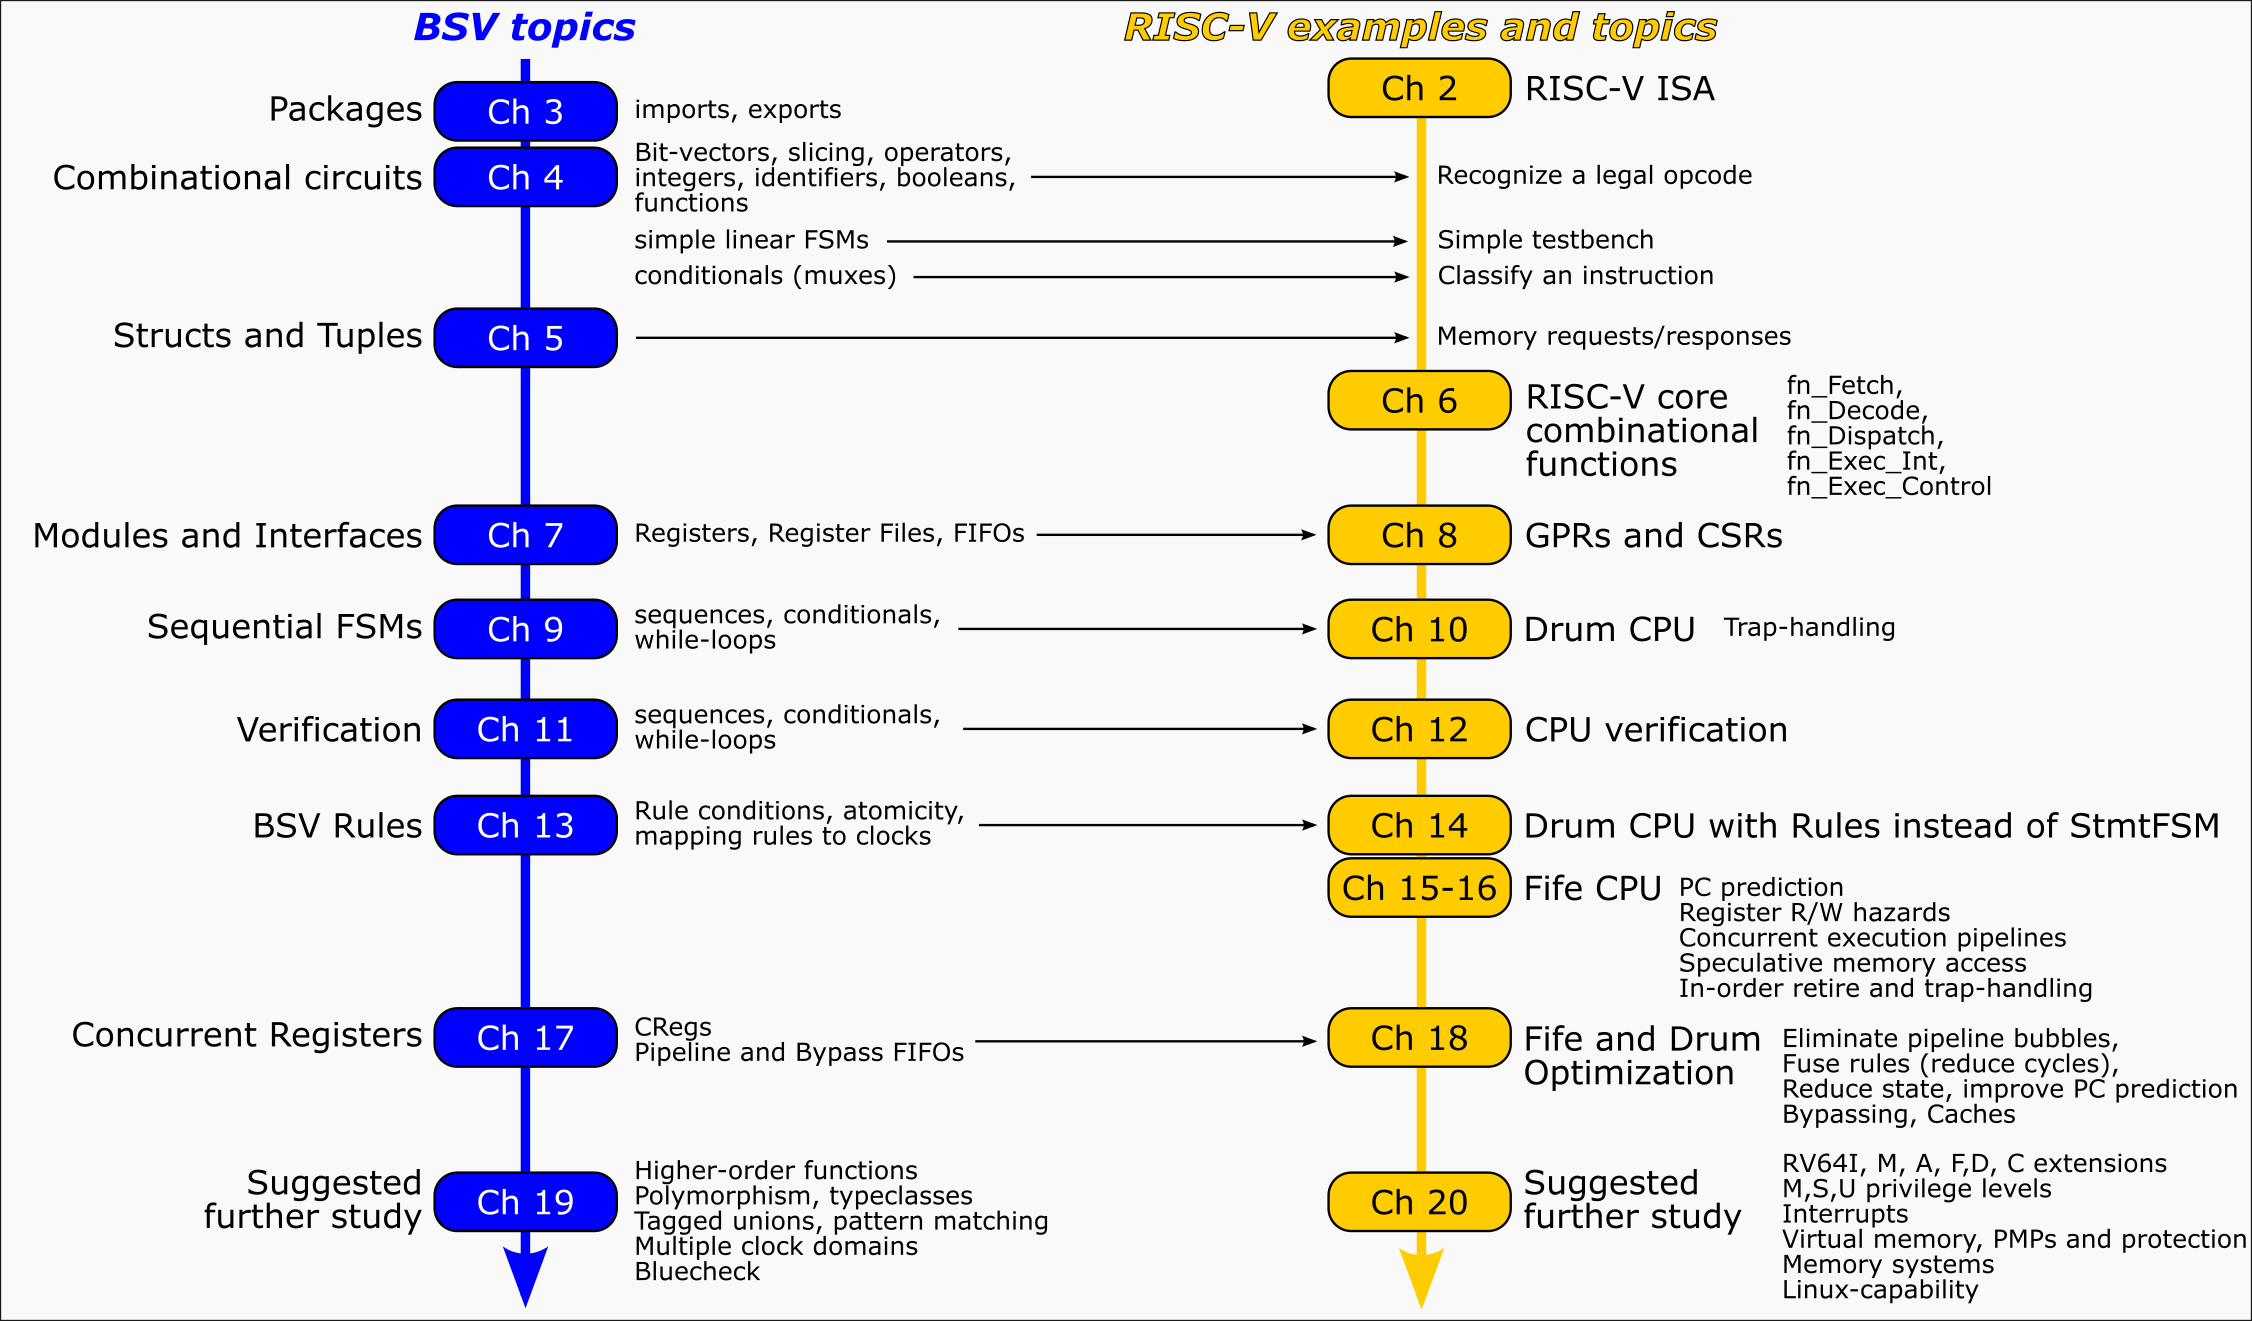
\includegraphics[height=0.825\textheight]{Fig_Chapter_Roadmap}}
\end{center}

\end{frame}

% ================================================================


% ================================================================

\begin{frame}
\frametitle{Flow of information between stages in Drum and Fife}

\footnotesize

\begin{center}
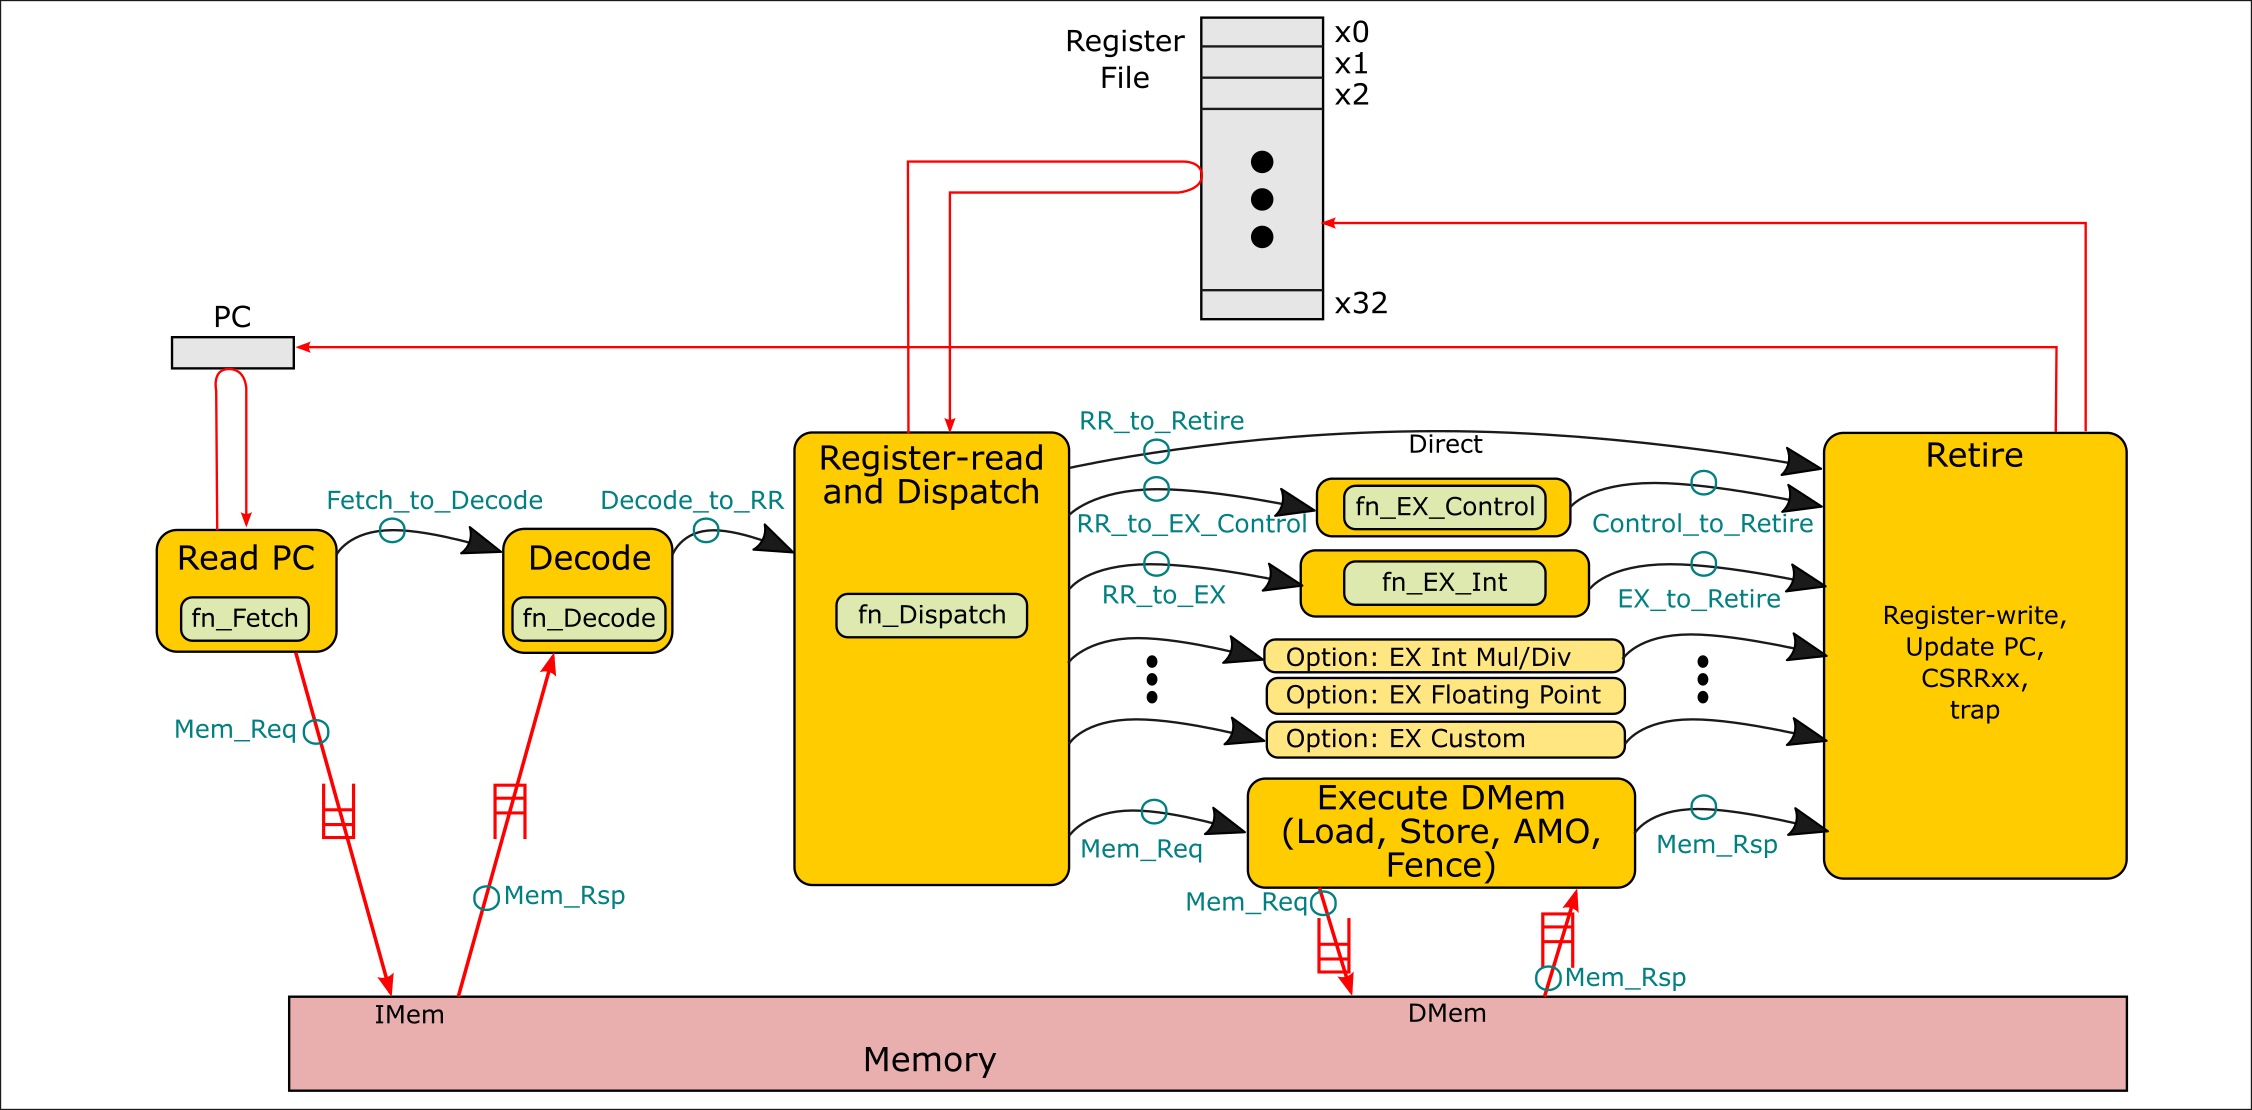
\includegraphics[height=0.6\textheight]{Fig_Instr_Exec_w_structs}
\end{center}

\end{frame}

% ================================================================

\begin{frame}
\frametitle{Table of Contents}

\tableofcontents

\end{frame}

% ****************************************************************

\section{Generic Information on Modules and Interfaces}

% ================================================================

\begin{frame}

\begin{center}
  {\LARGE Generic Information on Modules and Interfaces}
\end{center}

\end{frame}

% ================================================================

\begin{frame}
\frametitle{{\BSV}: What's in an Interface Declaration?}

\begin{center}
\includegraphics[width=\textwidth]{../Figures/Fig_BSV_whats_in_an_interface_decl}
\end{center}

\end{frame}

% ================================================================

\begin{frame}
\frametitle{{\BSV}: What's in a Module Declaration?}

\begin{center}
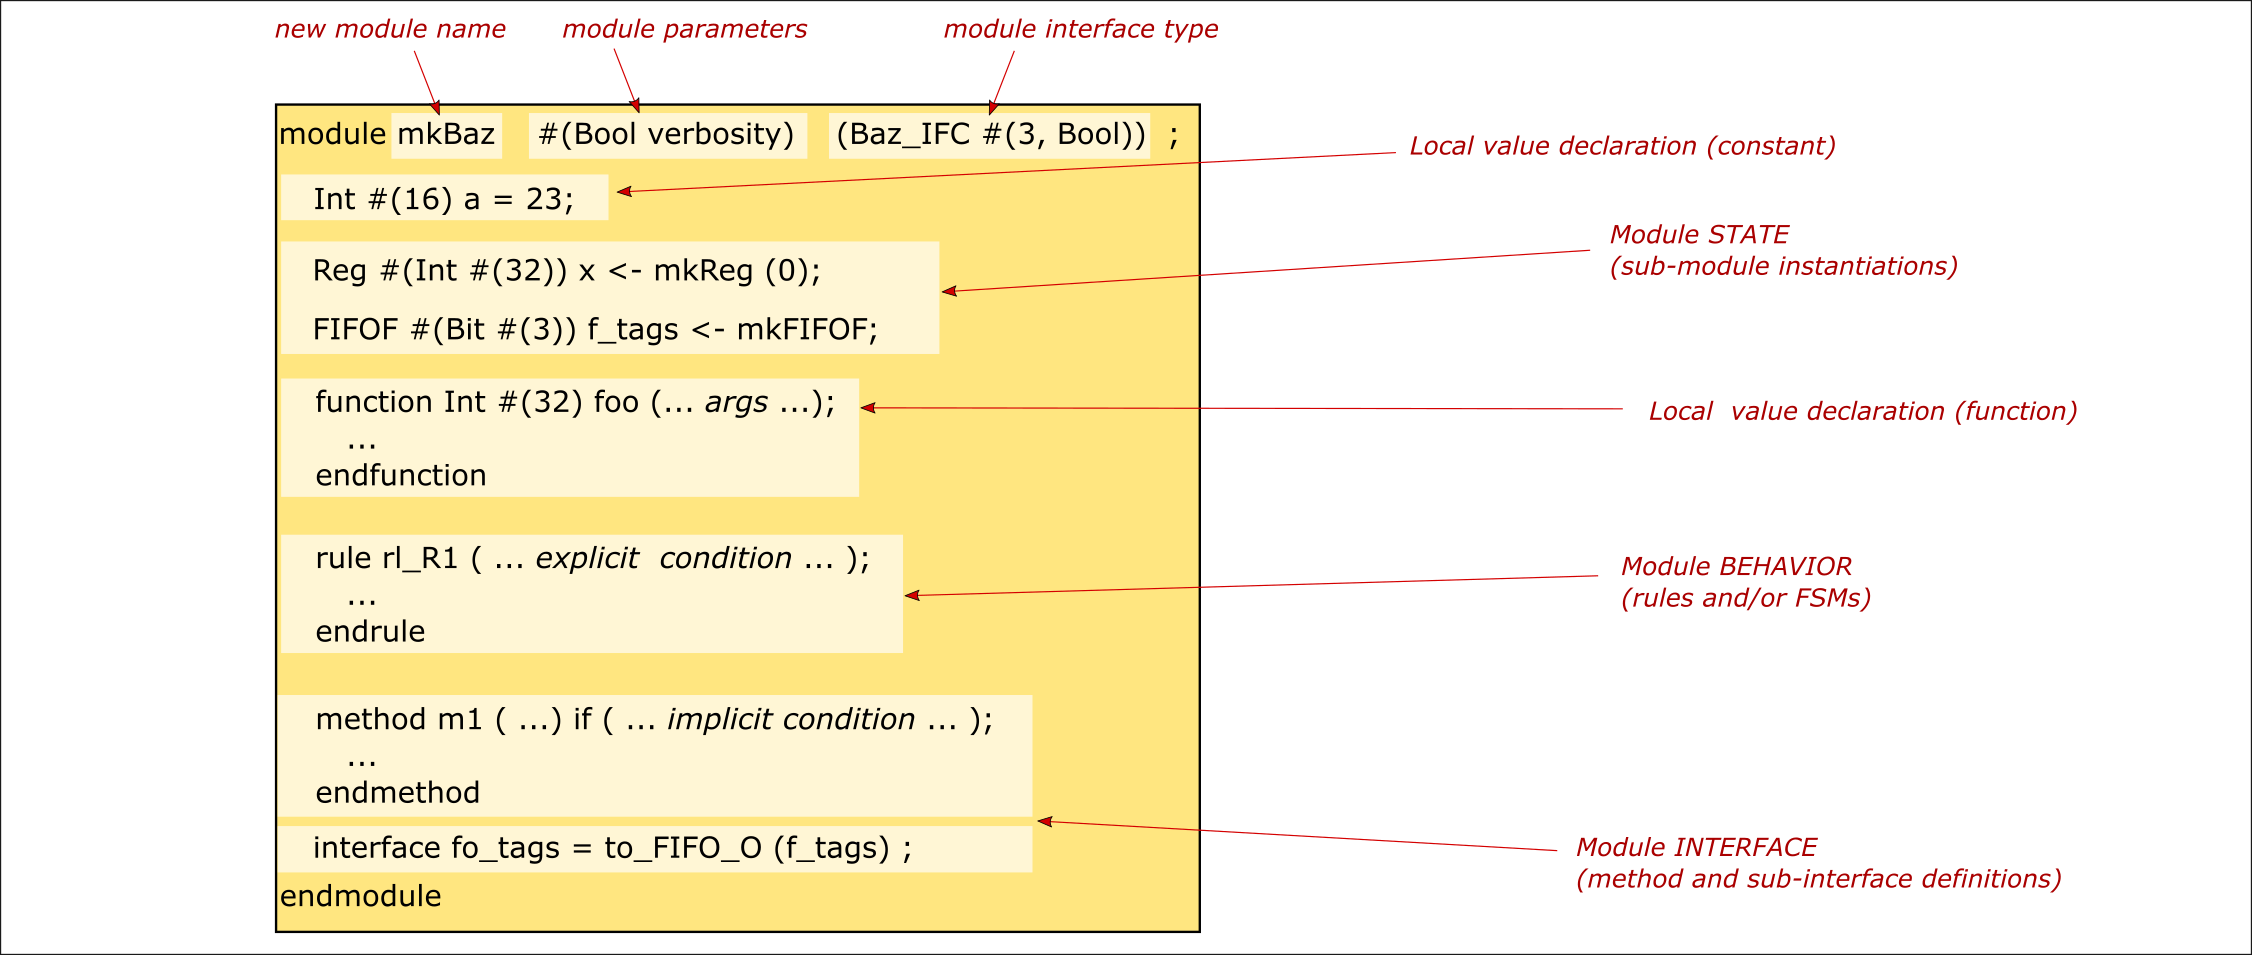
\includegraphics[width=\textwidth]{../Figures/Fig_BSV_whats_in_a_module_decl}
\end{center}

\end{frame}

% ================================================================

\begin{frame}
\frametitle{{\BSV}: What's in a Rule?}

\begin{center}
\includegraphics[width=\textwidth]{../Figures/Fig_BSV_whats_in_a_rule}
\end{center}

\end{frame}

% ================================================================

\begin{frame}
\frametitle{{\BSV}: What's in an Interface Definition?}

\begin{center}
\includegraphics[width=\textwidth]{../Figures/Fig_BSV_whats_in_an_interface_def}
\end{center}

\end{frame}

% ================================================================

\begin{frame}
\frametitle{{\BSV}: Static elaboration}

\begin{center}
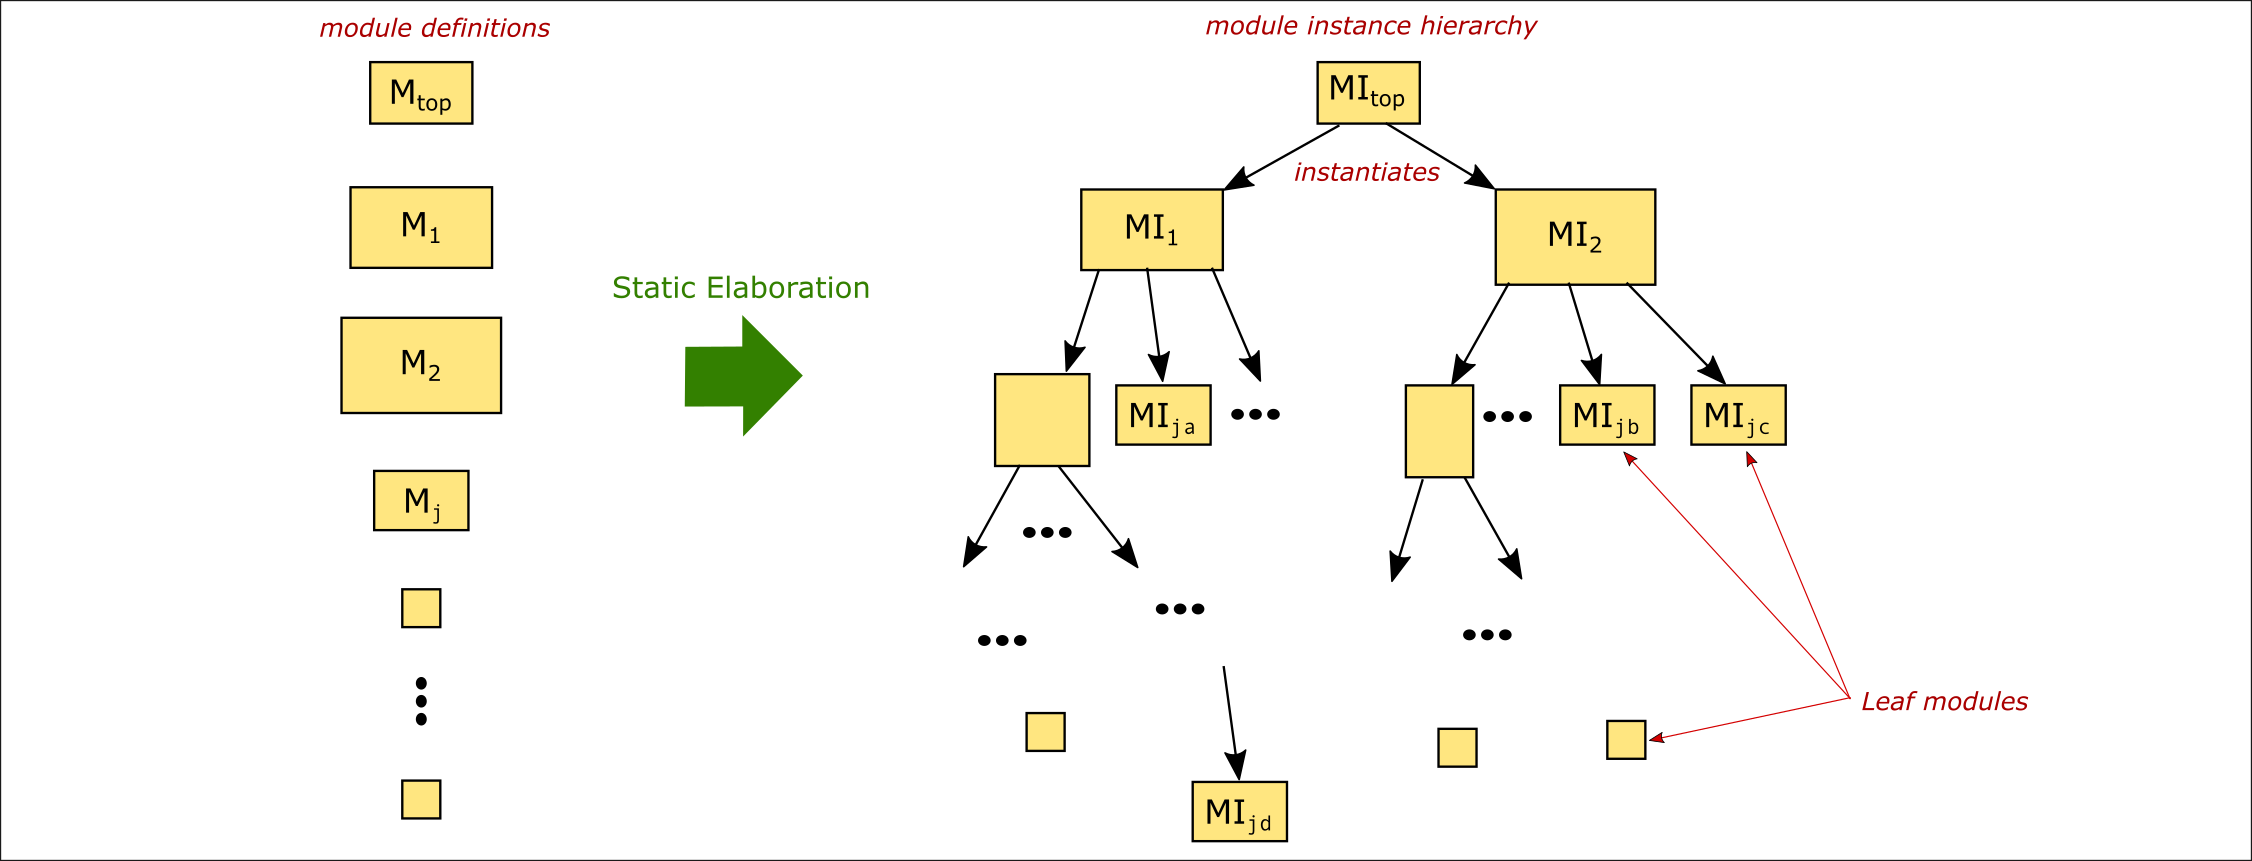
\includegraphics[width=\textwidth]{../Figures/Fig_BSV_static_elaboration}
\end{center}

\end{frame}

% ================================================================

\begin{frame}
\frametitle{{\BSV}: Module interaction}

\begin{center}

\includegraphics[width=\textwidth]{../Figures/Fig_BSV_module_interaction}
\end{center}

\end{frame}

% ================================================================

\begin{frame}[fragile]
\frametitle{{\BSV}: Generating a Verilog module for a {\tt BSV} module}

\footnotesize

By default, wherever we have an instantiation of a module FOO, the
{\bsc} compiler \emph{inlines} the corresponding FOO module definition
at that place.

\vspace{1ex}

As a consequence, there will be no trace of module FOO in the generated Verilog.

\vspace{4ex}

We can place a ``\verb|(* synthesize *)|'' attribute just before a module declaration:

\begin{Verbatim}[frame=single]
(* synthesize *)
module mkCPU (CPU_IFC);
   ...
endmodule
\end{Verbatim}

This
\begin{itemize}
 \item Makes {\bsc} generate a Verilog module for {\tt mkCPU}

 \item Wherever {\tt mkCPU} is instantiated, {\bsc} will instantiate
       that Verilog module there, instead of inlining it.

\end{itemize}

\vspace{2ex}

CAVEAT: all {\BSV} modules can be inlined, but not all {\BSV} modules
can be converted into Verilog.  Briefly, the modules inputs and
outputs all need to be representable as wires carrying bit-vectors.

\end{frame}

% ================================================================

\begin{frame}
\frametitle{{\BSV}: Hardware interfaces}

\footnotesize

General scheme for all {\BSV} Hardware interfaces: \\
\hmm (wires/buses) for {\tt ActionValue\#(t)}, {\tt Action} and value methods:

\vspace{2ex}

\begin{center}
\includegraphics[width=\textwidth]{Fig_Interface_Buses}
\end{center}

\end{frame}

% ****************************************************************

\section{Registers}

% ================================================================

\begin{frame}

\begin{center}
  {\LARGE Registers}
\end{center}

\end{frame}

% ================================================================

\begin{frame}[fragile]
\frametitle{{\BSV} library: Registers}

\footnotesize

Registers are the simplest ``state elements'' (entities that have
state, {\ie} that store or retain values over time).

\vspace{2ex}

In {\BSV}, registers are treated just like user-defined modules. \\
(unlike Verilog/System Verilog, where registers are special primitives, not modules).

\vspace{2ex}

The pre-defined ``{\tt Reg}'' interface is an interface with two methods:

\begin{Verbatim}[frame=single]
interface Reg #(t);
   method t _read();
   method Action _write (t x);
endinterface
\end{Verbatim}

\vspace{1ex}

Registers are instantiated just like user-defined modules:

\begin{Verbatim}[frame=single]
    // register with reset value
   Reg #(Bit #(XLEN))  rg_pc <- mkReg (0);

   // uninitialized register (unspecified reset value)
   Reg #(Bit #(XLEN))  rg_pc <- mkRegU;
\end{Verbatim}

\vspace{2ex}

In {\BSV}, registers are strongly-typed. \\
A \verb|Reg #(Bit #(XLEN))| cannot contain a {\tt Bool} value,
  or a \verb|Mem_Req| value,
  or ... any value whose type is not \verb|Bit #(XLEN)| \\
(unlike Verilog/System Verilog, where all registers just hold bit-vectors).

\end{frame}

% ================================================================

\begin{frame}[fragile]
\frametitle{{\BSV}: Syntactic shorthands for reading and writing registers}

\footnotesize

Because register access is so frequent, {\BSV} provides some syntactic
shorthands for regsiter-method invocations:

\vspace{2ex}

\begin{center}
 \begin{minipage}{0.25\textwidth}
  \begin{Verbatim}[frame=single]
  rg_pc + 4
  \end{Verbatim}
 \end{minipage}
 \hm is shorthand for \hm
 \begin{minipage}{0.35\textwidth}
  \begin{Verbatim}[frame=single]
  rg_pc._read + 4
  \end{Verbatim}
 \end{minipage}

 \begin{minipage}{0.25\textwidth}
  \begin{Verbatim}[frame=single]
  rg_pc <= v
  \end{Verbatim}
 \end{minipage}
 \hm is shorthand for \hm
 \begin{minipage}{0.35\textwidth}
  \begin{Verbatim}[frame=single]
  rg_pc._write (v);
  \end{Verbatim}
 \end{minipage}
\end{center}

\PAUSE{\vspace{4ex}}

Example:

\vspace{1ex}

\begin{center}
 \begin{minipage}{0.25\textwidth}
  \begin{Verbatim}[frame=single]
  rg_pc <= rg_pc + 4;
  \end{Verbatim}
 \end{minipage}
 \hm is shorthand for \hm
 \begin{minipage}{0.35\textwidth}
  \begin{Verbatim}[frame=single]
  rg_pc._write (rg_pc._read + 4);
  \end{Verbatim}
 \end{minipage}
\end{center}

\end{frame}

% ****************************************************************

\section{Register Files}

% ================================================================

\begin{frame}

\begin{center}
  {\LARGE Register Files}
\end{center}

\end{frame}

% ================================================================

\begin{frame}[fragile]
\frametitle{{\BSV} library: Register Files}

\footnotesize

A Register File module is an array of registers.

\vspace{4ex}

Unlike a collection of individual registers, where we can
simultaneously read and write all registers, a register file is
organized and accessed like a memory through a read and write
interface.

\vspace{2ex}

\begin{itemize}

 \item To read the $j^{th}$ register, we must give it the register
       index $j$ (like a ``memory address'').

       The standard {\BSV} register file module has 5 read-ports,
       {\ie} up to 5 registers can be read simultaneously (in RISC-V,
       we need to read at least two registers simultaneously).

 \PAUSE{\vspace{2ex}}

 \item To write the $j^{th}$ register, we must give it the register
       index $j$ and the value $v$ to be written.

\end{itemize}

\PAUSE{\vspace{2ex}}

A synthesis tool may implement a register file using an SRAM, instead
of using random registers and muxes.

\end{frame}

% ================================================================

\begin{frame}[fragile]
\frametitle{{\BSV} library: Register Files}

\footnotesize

(See ``Bluespec Compiler (BSC) Libraries Reference Guide'', Section ``3.1.1 Register File''.)

\vspace{2ex}

The {\tt RegFile} interface:

\begin{Verbatim}[frame=single]
interface RegFile #(type index_t, type data_t);
   method Action upd (index_t addr, data_t d);      // write a register
   method data_t sub (index_t addr);                // read a register
endinterface: RegFile
\end{Verbatim}

\vspace{2ex}

``\verb|index_t|'' is the type for the index (for RISC-V, with 32
registers, we use \verb|Bit#(5)|).

``\verb|data_t|'' is the type of value stored in each of the
registers (for RISC-V, this is \verb|Bit#(XLEN)|.

\vspace{1ex}

{\BSV} register files are strongly typed, just like individul registers. \\
(unlike Verilog/SystemVerilog, where register files just hold bit-vectors).

\vspace{2ex}

Example of instantiating a 31-register register-file module:

\begin{Verbatim}[frame=single]
RegFile #(Bit #(5), Bit #(XLEN)) gprs <- mkRegFile (1, 31);
\end{Verbatim}

Example of instantiating a 32-register register-file module:

\begin{Verbatim}[frame=single]
RegFile #(Bit #(5), Bit #(XLEN)) gprs <- mkRegFileFull;
\end{Verbatim}

\end{frame}

% ****************************************************************

\section{FIFOs}

% ================================================================

\begin{frame}

\begin{center}
  {\LARGE FIFOs}
\end{center}

\end{frame}

% ================================================================

\begin{frame}[fragile]
\frametitle{{\BSV} library: FIFOs}

\footnotesize

FIFO modules hold \emph{queues} of items. \\
We can \emph{enqueue} an item on one end of a FIFO. \\
At the other end of the FIFO, we can examine the first element, and/or
\emph{dequeue} (remove) an item.

\PAUSE{\vspace{2ex}}

A pre-defined FIFO interface in the {\BSV} library:
\begin{Verbatim}[frame=single]
interface FIFOF #(t);
   method Bool   notEmpty;
   method Bool   notFull;
   method t      first;
   method Action deq;
   method Action enq (t x);
   method Action clear;        // Empty the FIFO
endinterface
\end{Verbatim}

``{\tt t}'' specifies the type of the elements that the FIFO carries. \\
{\BSV} FIFOs are strongly typed.  A \verb|FIFOF #(Mem_Req)| cannot carry \verb|Mem_Rsp|s.

\PAUSE{\vspace{2ex}}

Any actual hardware FIFO module will have a fixed maximum
capacity (the number of items that it can hold in the queue) after
which it becomes ``full''.

\vspace{1ex}

Different FIFO modules with the \verb|FIFOF #(t)| interface may have
different capacities.

\end{frame}

% ================================================================

\begin{frame}[fragile]
\frametitle{{\BSV} library: FIFO modules}

\footnotesize

Instantiating FIFO modules: Examples:
\begin{Verbatim}[frame=single]
   FIFOF #(Mem_Req) f_to_IMem   <- mkFIFOF;
   FIFOF #(Mem_Rsp) f_from_IMem <- mkFIFOF;

   FIFOF #(RR_to_Retire)  f_RR_to_Retire <- mkSizedFIFOF (8);
\end{Verbatim}

\end{frame}

% ================================================================

\begin{frame}[fragile]
\frametitle{{\BSV} library: A useful help-function}

\footnotesize

A useful function combining the {\tt first} and {\tt deq} methods:
\begin{Verbatim}[frame=single]
function ActionValue #(t) pop (FIFOF #(t) fifo);
   actionvalue
      let x = fifo.first;
      fifo.deq;
      return x;
   endactionvalue
endfunction
\end{Verbatim}

\vspace{4ex}

\begin{center}
So \hmm
\begin{minipage}{0.3\textwidth}
\begin{Verbatim}[frame=single]
   let y <- pop (fifo);
\end{Verbatim}
\end{minipage}
\hmm is equivalent to \hmm
\begin{minipage}{0.3\textwidth}
\begin{Verbatim}[frame=single]
   let y fifo.first;
   fifo.deq;
\end{Verbatim}
\end{minipage}
\end{center}

\end{frame}

% ================================================================

\begin{frame}[fragile]
\frametitle{{\BSV} library: {\tt SemiFIFOF} interfaces for each end of a FIFO}

\footnotesize

When a FIFO is used for communication between two modules, it is
enqueued in one module and dequeued in the other.  Conceptually, each
module uses only one end of the FIFO.

\vspace{1ex}

For this, it is useful to define interfaces representing one end of a FIFO:

\vspace{1ex}

Input end (where we enqueue):
\begin{Verbatim}[frame=single]
interface FIFOF_I #(t);
   method Bool notFull();
   method Action enq (t x);
endinterface
\end{Verbatim}

\vspace{1ex}

Output end (where we dequeue), and associated \verb|pop_O| function:

\begin{minipage}[t]{0.3\textwidth}
\begin{Verbatim}[frame=single]
interface FIFOF_O #(t);
   method Bool notEmpty();
   method t first();
   method Action deq();
endinterface
\end{Verbatim}
\end{minipage}
\hm
\begin{minipage}[t]{0.6\textwidth}
\begin{Verbatim}[frame=single]
function ActionValue #(t) pop_O (FIFOF_O #(t) fo);
   actionvalue
      let x = fo.first;
      fo.deq;
      return x;
   endactionvalue
endfunction
\end{Verbatim}
\end{minipage}

\end{frame}

% ================================================================

\begin{frame}[fragile]
\frametitle{{\BSV} library: transforming a {\tt FIFOF} interface into a {\tt FIFOF\_O} interface}

\footnotesize

\begin{Verbatim}[frame=single]
function FIFOF_O #(t) to_FIFOF_O (FIFOF #(t) f);
   interface FIFOF_O #(Mem_Req) fo_IMem_req;
      method Bool notEmpty();
         return f.notEmpty;
      endmethod

      method t first();
         return f.first;
      endmethod

      method Action deq();
         f.deq;
      endmethod
   endinterface
endfunction
\end{Verbatim}

\PAUSE{\vspace{4ex}}

We can write a similar function transforming a {\tt FIFOF} interface
into a {\tt FIFOF\_I} interface.

\end{frame}

% ================================================================

\begin{frame}
\frametitle{\EmojiExercise \hmm Exercise break}

Please see Appendix E, Section Ex-07-A-Modules-Interfaces.

\end{frame}

% ================================================================

\begin{frame}[fragile]
\frametitle{{\BSV} library: Connecting FIFOs}

\footnotesize

\begin{center}
\begin{minipage}{0.4\textwidth}
\begin{Verbatim}[frame=single]
interface Fetch_IFC;
   interface FIFOF_O #(F_to_D)
             fo_Fetch_to_Decode;
   ...
endinterface
\end{Verbatim}
\end{minipage}
\hmm
\begin{minipage}{0.4\textwidth}
\begin{Verbatim}[frame=single]
interface Decode_IFC;
   interface FIFOF_I #(F_to_D)
             fi_Fetch_to_Decode;
   ...
endinterface
\end{Verbatim}
\end{minipage}
\end{center}

\vspace{2ex}

In the parent CPU module:

\begin{Verbatim}[frame=single]
module mkCPU (CPU_IFC);
   ...
   // Instantiate Fetch and Decode stages
   Fetch_IFC   stage_F  <- mkFetch;
   Decode_IFC  stage_D  <- mkDecode;
   ...
   // Connect the Fetch_to_Decode flow
   Empty eifc <- mkConnection (stage_F.fo_Fetch_to_Decode, stage_D.fi_Fetch_to_Decode);
   ...
endmodule
\end{Verbatim}

\end{frame}

% ================================================================

\begin{frame}[fragile]
\frametitle{{\BSV} library: {\tt mkConnection}}

\footnotesize

{\tt mkConnection} is just another module, and could easily be written
by the user if it were not pre-defined for the \verb|FIFOF_O| and
\verb|FIFOF_I| interfaces.

\begin{Verbatim}[frame=single]
module mkConnection #(FIFOF_O #(Fetch_to_Decode) f,    // module argument
                      FIFOF_I #(Fetch_to_Decode) d)    // module argument
                    (Empty);                           // module interface
   rule rl_connect;
       let x = f.first;
       f.deq;
       d.enq (x);
   endrule
endmodule
\end{Verbatim}

\PAUSE{\vspace{4ex}}

In general, whenever there is pair of interface types that can and are
frequently connected, we recommend defining {\tt mkConnection} for
those interfaces.

\end{frame}

% ================================================================

\begin{frame}[fragile]
\frametitle{{\BSV} library: {\tt mkConnection}}

\footnotesize

Shorthand: in this line:

\vspace{1ex}

\begin{Verbatim}[frame=single]
   Empty eifc <- mkConnection (stage_F.fo_Fetch_to_Decode, stage_D.fi_Fetch_to_Decode);
\end{Verbatim}

\vspace{1ex}

Because this is an empty interface (has no methods) and is therefore
never used, in {\BSV} we can just omit the ``{\tt Empty eifc <-}''
part:

\vspace{1ex}

\begin{Verbatim}[frame=single]
   mkConnection (stage_F.fo_Fetch_to_Decode, stage_D.fi_Fetch_to_Decode);
\end{Verbatim}

\end{frame}

% ****************************************************************

% -*- mode: fundamental -*-

% Slides accompanying "Learn RISC-V CPU Implementation and BSV" book
% Copyright (c) 2024 Rishiyur S. Nikhil, All Rights Reserved

% This is a postamble shared by all the slide decks

% ================================================================

\begin{frame}

\begin{center}
  {\LARGE End}
\end{center}

\end{frame}

% ================================================================


% ****************************************************************

\end{document}
